\documentclass[12pt]{article} % This command is used to set the type of document you are working on such as an article, book, or presenation

% \usepackage{geometry} % This package allows the editing of the page layout
% \usepackage{amsmath}  % This package allows the use of a large range of mathematical formula, commands, and symbols
% \usepackage{graphicx}  % This package allows the importing of images
\usepackage[T1]{fontenc}
\usepackage{blindtext}
\usepackage[]{algorithm2e}
\usepackage{graphicx}
\usepackage{float}
\usepackage{amsfonts, amssymb, amsmath}
\usepackage[utf8]{inputenc}
\parindent 0px

\graphicspath{ {Results/Graficas} }
% \usepackage[T1]{fontenc}
\title{Comparativa de Algoritmos de Ordenamiento\\Estructura de Datos y Algoritmos}
\date{Agosto 2023}
\author{Jesus Alpaca Rendon}     
\begin{document}
\maketitle
\section{Introduccion}
El presente informe muestra la comparativa de tiempos de ejecucion realizada entre 5 algoritmos de ordenamiento como son: Binary Insertion Sort, Bubble sort, Quick sort, Selection sort y Merge sort.
Implementados en 3 diferentes lenguajes de programacion: Python, Golang y C++. Los algoritmos fueron sometidos a pruebas para obtener un tiempo promedio de ejecucion y ver los resultados
en tablas comparativas y graficos con los resultados para determinar el performance de los algoritmos y lenguajes.
\section{Algoritmos}
Los algoritmos seleccionados para el presente trabajo de investigacion son los siguientes:

* Binary Insertion Sort

* Bubble sort

* Quick sort

* Selection sort

* Merge Sort

\begin{enumerate}
    \item Binary Insertion Sort
        
        Este algoritmo es una combinacion de 2 algoritmos existentes: Binary Search y Insertion Sort,
        Esta combinacion nos permite ordenar una lista de n valores, el cual se constituye en un inicio de un bucle que nos permitira recorrer todo el array
        seleccionando el segundo elemento, ya que se considera el primero como ordenado, una vez seleccionado, aplicaremos la busqueda binaria, Cabe resaltar que la busqueda binaria funciona correctamente si la lista esta ordenada.
        En este caso la busqueda binaria solo se aplicara al lado izquierdo del array ya que es la parte considerada ordenada. Comparamos el valor siguiente i+1 con el punto medio de la lista ordenada,
        y se verifica si es mayor o menor, en caso de ser mayor se coloca en al derecha y caso contrario a la izquierda. En el mejor de los casos, el algoritmo de Insertion Sort puede tener una sola comparacion, pero en el peor
        de los casos puede tener n comparaciones, y en el caso de Binary Insertion sort, reducimos el maximo de casos, ya que se reduce a log n comparaciones como maximo .Estos pasos se repiten por cada elemento dejandonos en un inicio una complejidad de O(n),
        la cual con la complejidad de Binary Search de nos da una complejidad de O(n log n), sin embargo, no se esta considerando el movimiento que se da a los items en caso tengamos numeros peque;os al final, para esto, tendria que recorrer
        n posiciones hasta colocarlo en su lugar, lo cual incrementaria la complejidad, quedando lo siguiente: Binary Search + movimiento de items = O(log n) + O(n). Si ahora colocamos la complejidad de Insert Sort, nos quedaria de esta manera:
        O(n) x (O(log n) + O(n)) = O(n log n) + O(n2). Como complejidad final del algoritmo Binary Insertion Sort tendriamos O(n2).

        \begin{figure}[H]
        \centering
        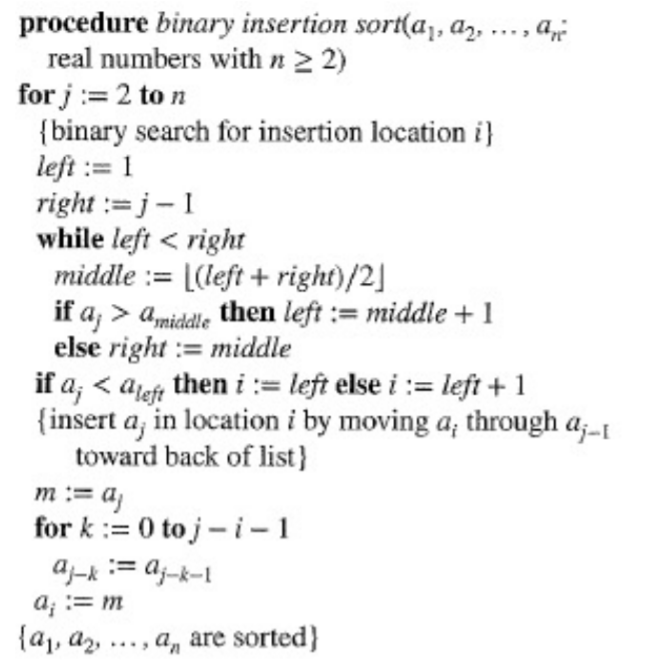
\includegraphics[width=8cm, height=8cm]{binaryinsertionsort_pseudocode}
        \caption{Binary Insertion Sort Algorithm}
        \end{figure}

    \item Bubble Sort
    
          Este algoritmo realiza el ordenamiento o reordenamiento de una lista a de n valores, en este caso de n términos numerados del 0 al n-1; consta de dos bucles anidados, uno con el índice i, que da un tamaño menor al recorrido de la burbuja en sentido inverso de 2 a n, y un segundo bucle con el índice j,
          con un recorrido desde 0 hasta n-i, para cada iteración del primer bucle, que indica el lugar de la burbuja. La burbuja son dos términos de la lista seguidos, j y j+1, que se comparan: si el primero es mayor que el segundo sus valores se intercambian.

          \begin{algorithm}[H]
              \KwData{$a_{1}$,$a_{2}$,$a_{3}$,$a_{4}$...$a_{(n-1)}$}
              \KwResult{ordered list}
              initialization\;
              \For{$i$ \KwTo n-1}{
                  \For{$j$ \KwTo n-i-1}{
                      \If{$a_{j}$ > $a_{j+1}$}{
                          go to next section\;
                          $aux\gets a_{j}$\;
                          $a_{j}\gets a_{j+1}$\;
                          $a_{j+1}\gets aux$\;                          
                      }
                  }
              }              
              \caption{Bubble Algorithm}
          \end{algorithm}

    \item Quick Sort
    
          Es uno de los algoritmos mas rapidos. Tiene un elemento muy importante para su ejecucion la cual es la seleccion del pivote. El pivote es el elemento desde el cual nosotros dividiremos la lista.
          Quicksort es un algoritmo de divide y venceras y el pivote es muy importante, incluso su seleccion influye en su complejidad. Principalmente el algoritmo toma el pivote, divide la lista y empieza a analizar:
          Si encuentra un numero menor que el pivote, lo colocara a su izquierda, caso contrario a la derecha, adicionalmente se debe tener punteros al inicio y al final.
          Por cada array que se forma se debe escoger un pivote,al final tendremos una lista ordenada sin necesidad de aplicar una mezcla como lo usa el merge sort.
          La complejidad del algoritmo es de O(nlogn) el cual es comparado con merge sort, sin embargo hay que tener en cuenta que el peor de los casos de este algoritmo es cuando
          tenemos una lista ordenada y se selecciona como pivote uno de los extremos, dandonos una complejidad en este caso de O(n2)

        \begin{figure}[H]
        \centering
        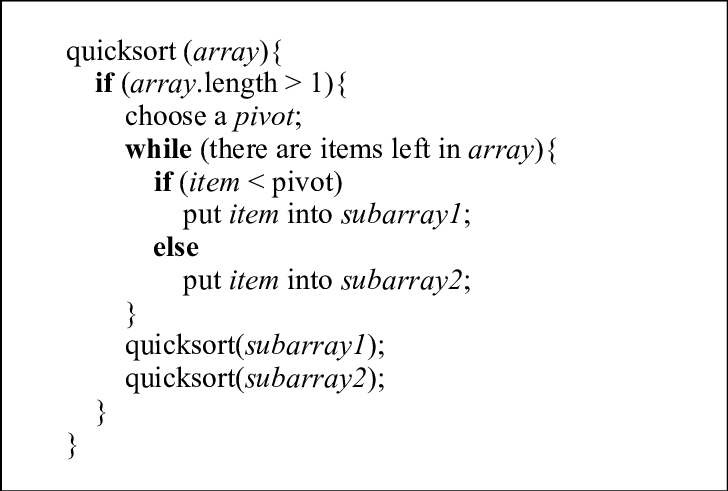
\includegraphics[width=9cm, height=9cm]{quicksort_pseudocode}
        \caption{Quick Sort Algorithm}
        \end{figure}

    \item Selection Sort
    
          Este algoritmo tiene una complejidad de O(n2), por lo que no es uno de los mas rapidos, el algoritmo empieza determinando 2 elementos claves
          los cuales son: el minimo actual y el item actual, para ello inicia en la posicion inicial. Durante cada iteracion, va seleccionando el item minimo
          de la lista desordenada y lo mueve a la posicion ordenada, cuando encuentra el minimo, lo intercambia con la posicion del item seleccionado. Es por esta razon que
          tiene una complejidad alta ya que al intercambiarlo, en caso que sea el item minimo consecuente, tendra que recorrer en el peor de los casos n veces para hacer el intercambio

        \begin{figure}[H]
        \centering
        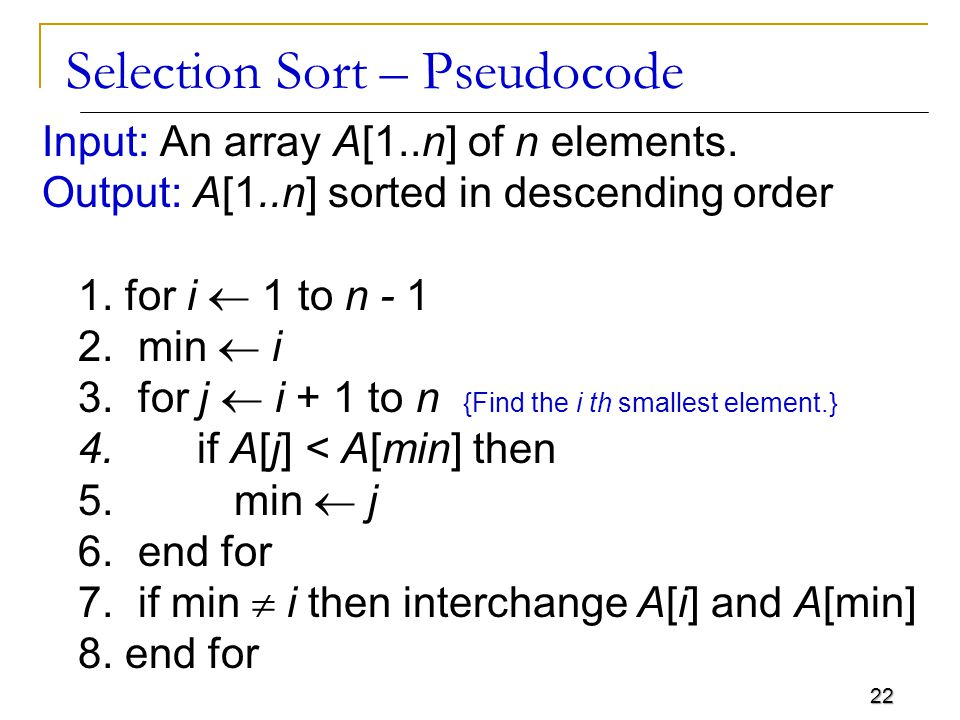
\includegraphics[width=6cm, height=8cm]{selectionsort_pseudocode}
        \caption{Selection Sort Algorithm}
        \end{figure}

    \item Merge Sort
    
          El algoritmo Merge Sort se puede representar en 2 partes: la funcion MergeSort que realiza la division de una lista de numeros en 2 partes, siendo el punto medio la parte donde se divide, y la funcion mezclar
          Que es la que se encargara de realizar la logica donde se ordenara 2 listas que recibe como parametro y hacer una mezcla entre ellas. El algoritmo Merge Sort es uno de los algoritmos mas rapidos de ordenamiento,
          ya que nos permite reducir la lista en partes iguales y realizar mezclas sucesivas. Cuando la longitud de un array es 1, se considera ordenado y retorna, en caso de lista de n elementos, la comparacion se hace en parejas
          es decir, empieza a comparar uno a uno los elementos iniciales de cada lista, creando una lista temporal donde tendremos la nueva lista mezclada y ordenada. Si durante el proceso de comparacion, el indice supera
          la longitud de la lista, se toma los elementos restantes de la otra y se colocan en la nueva lista. 
          La complejidad de este algoritmo es de O(n log n), siendo la parte de la comparacion la que tome mas protagonismo ya que al momento de comparar las 2 listas, estas se recorren con sus respectivos indices
          iterando de uno en uno los elementos y comparandolos segun la posicion que esten.

        \begin{figure}[H]
        \centering
        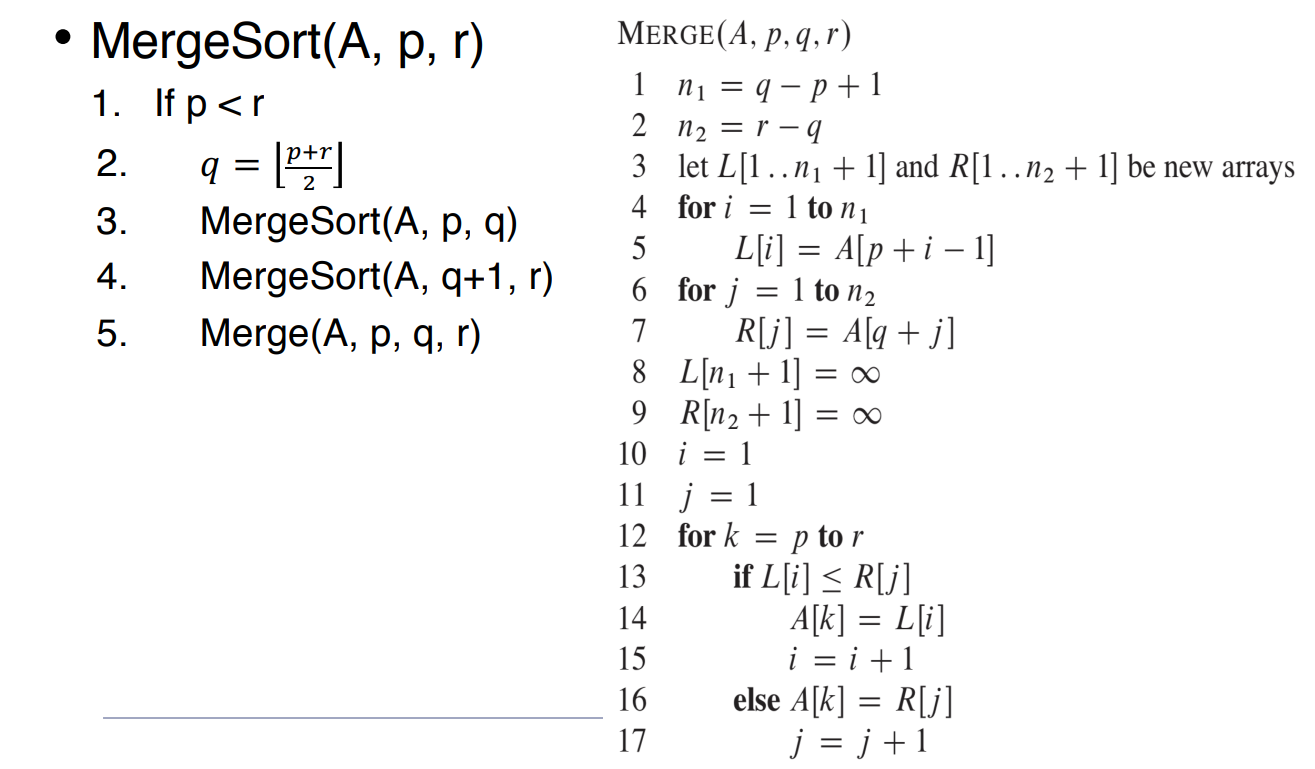
\includegraphics[width=12cm, height=8cm]{mergesort_pseudocode}
        \caption{Merge Sort Algorithm}
        \end{figure}

\end{enumerate}
\section{Implementacion}

Para la implementacion se trabajo en secuencia de la siguiente manera:
\begin{itemize}
    \item Se selecciono los algoritmos para trabajar y se busco su implementacion en los 3 lenguajes
    \item Se realizaron modificaciones para automatizar la ejecucion de las iteraciones con archivos txt que contenian listas de numeros de diferentes tamaños y que generara archivos con los resultados.
    \item Se creo scripts para generar los calculos del promedio y desviacion estandar por lenguaje y tamaño de la lista.
    \item Se genero un script para la generacion de los graficos comparativos por algoritmo y longitud de lista.
    \item Se genero una tabla comparativa general y otras por algoritmo para incluirse en el informe.
    \item Se desarrollo el presente informe en latex.
\end{itemize}

La implementacion del ejercicio se encuentra en el siguiente enlace de Github: https://github.com/Alpha004/MaestriaAyEDGrupo04
\section{Resultados}

Los resultados del informe se muestran en 5 tablas divididas por lenguajes donde cada una muestra las graficas correspondientes a las pruebas realizadas con los diferentes lenguajes
A continuacion se muestran las tablas comparativas y los graficos correspondientes por algoritmo:

\vspace{15cm}

BUBBLE SORT

\vspace{5mm}

\begin{table}[H]
    \def\arraystretch{1.3}
    \centering
    \begin{tabular}{|l|l|l|l|l|l|l|}
    \hline        
        DATOS & Python & ~ & C++ & ~ & Golang & ~ \\ \hline
        Cantidad & Promedio & Desv. Est. & Promedio & Desv. Est. & Promedio & Desv. Est. \\ \hline
        100 & 0.0018 & 0.0004 & 0.00054 & 0.000062 & 0.00034 & 0.000277 \\ \hline
        1000 & 0.1342 & 0.002401 & 0.0042 & 0.003119 & 0.001477 & 0.000428 \\ \hline
        2000 & 0.5764 & 0.043482 & 0.00923 & 0.000409 & 0.003846 & 0.000178 \\ \hline
        3000 & 1.232601 & 0.004318 & 0.020784 & 0.001754 & 0.007909 & 0.000213 \\ \hline
        4000 & 2.230502 & 0.042581 & 0.03684 & 0.00091 & 0.013814 & 0.000629 \\ \hline
        5000 & 3.5132 & 0.055782 & 0.058489 & 0.000285 & 0.021313 & 0.000226 \\ \hline
        6000 & 5.058199 & 0.163511 & 0.08836 & 0.001533 & 0.031634 & 0.0011 \\ \hline
        7000 & 6.958199 & 0.194601 & 0.119168 & 0.001122 & 0.046711 & 0.005821 \\ \hline
        8000 & 9.105999 & 0.21782 & 0.158906 & 0.001598 & 0.057926 & 0.000417 \\ \hline
        9000 & 11.510303 & 0.144547 & 0.209791 & 0.00918 & 0.075737 & 0.000391 \\ \hline
        10000 & 14.1332 & 0.269819 & 0.254562 & 0.00789 & 0.095036 & 0.000408 \\ \hline
        20000 & 56.44461 & 0.485198 & 1.088809 & 0.008167 & 0.442731 & 0.013076 \\ \hline
        30000 & 127.527399 & 0.335833 & 2.574614 & 0.057651 & 1.039052 & 0.015263 \\ \hline
        40000 & 226.8496 & 0.944975 & 4.670932 & 0.089209 & 1.89731 & 0.035354 \\ \hline
        50000 & 366.973335 & 15.659894 & 7.311926 & 0.038472 & 2.999633 & 0.039834 \\ \hline
    \end{tabular}
    \caption{Tabla de Promedios y Desviacion Estandar de los 3 lenguajes con Bubble Sort}
\end{table}

\vspace{9mm}


\begin{figure}[H]
    \centering
    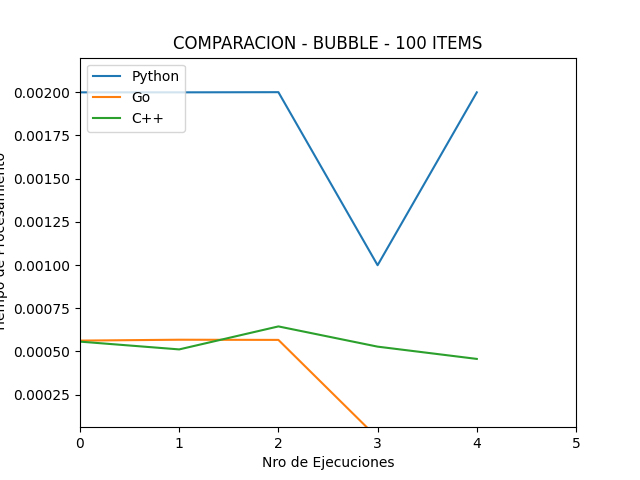
\includegraphics[width=\textwidth]{bubble_100}
    \caption{Bubble Sort - 100 items}
    \end{figure}
    
    \vspace{5mm}
    
    \begin{figure}[H]
    \centering
    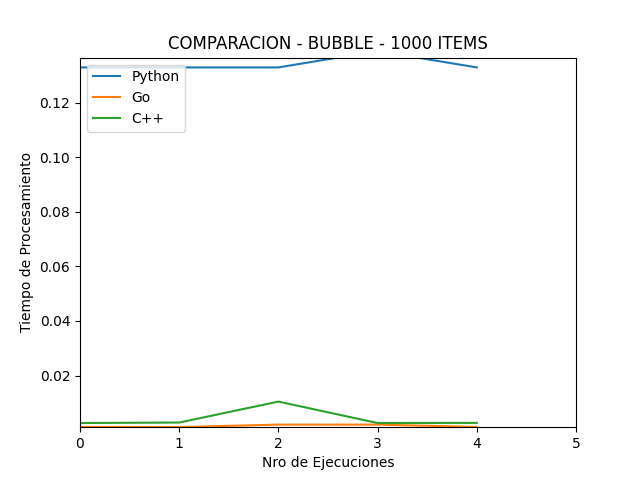
\includegraphics[width=\textwidth]{bubble_1000}
    \caption{Bubble Sort - 1000 items}
    \end{figure}
    
    \vspace{5mm}
    
    \begin{figure}[H]
    \centering
    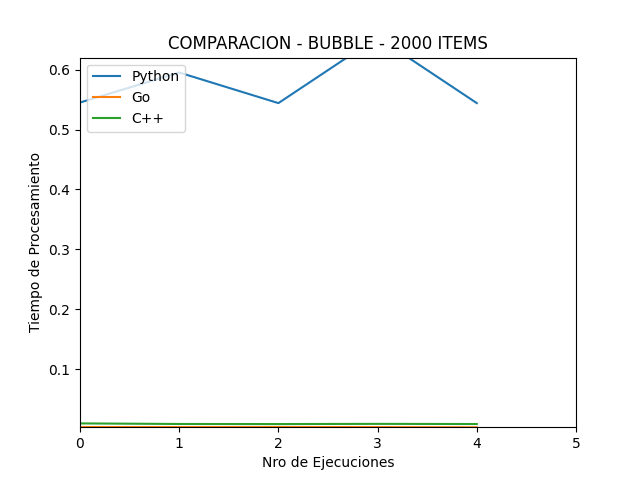
\includegraphics[width=\textwidth]{bubble_2000}
    \caption{Bubble Sort - 2000 items}
    \end{figure}
    
    \vspace{5mm}
    
    \begin{figure}[H]
    \centering
    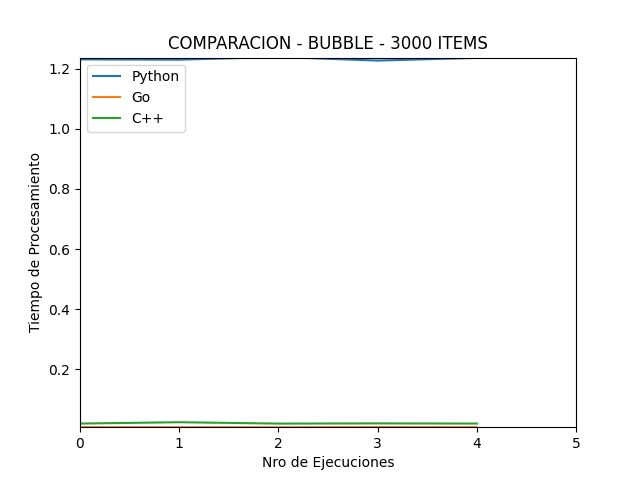
\includegraphics[width=\textwidth]{bubble_3000}
    \caption{Bubble Sort - 3000 items}
    \end{figure}
    
    \vspace{5mm}
    
    \begin{figure}[H]
    \centering
    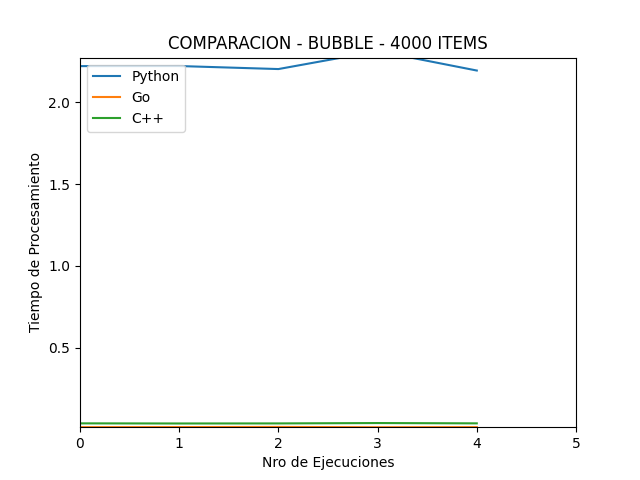
\includegraphics[width=\textwidth]{bubble_4000}
    \caption{Bubble Sort - 4000 items}
    \end{figure}

    \vspace{5mm}
    
    \begin{figure}[H]
    \centering
    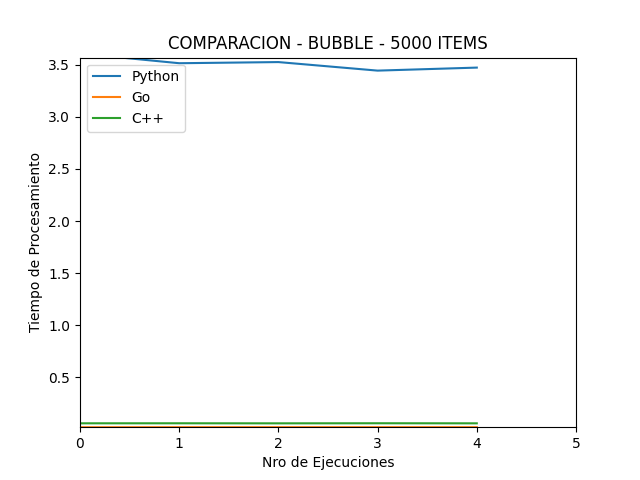
\includegraphics[width=\textwidth]{bubble_5000}
    \caption{Bubble Sort - 5000 items}
    \end{figure}

    \vspace{5mm}
    
    \begin{figure}[H]
    \centering
    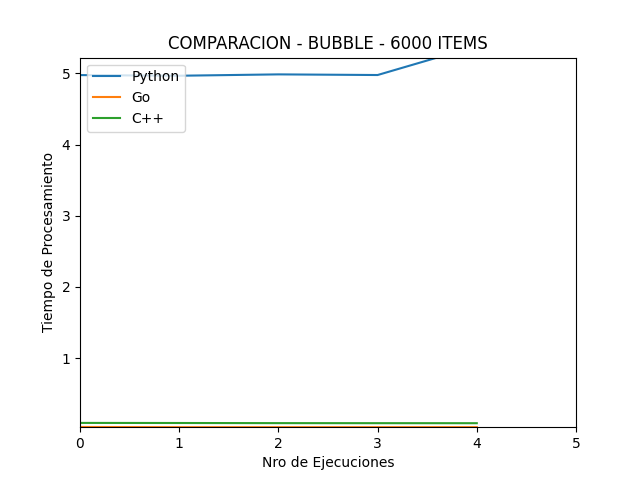
\includegraphics[width=\textwidth]{bubble_6000}
    \caption{Bubble Sort - 6000 items}
    \end{figure}

    \vspace{5mm}
    
    \begin{figure}[H]
    \centering
    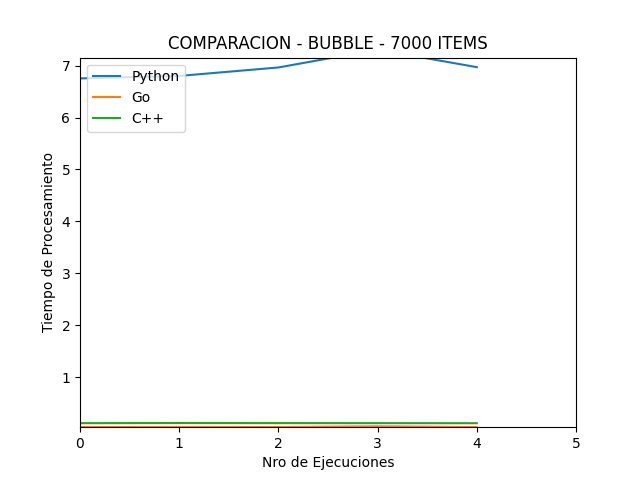
\includegraphics[width=\textwidth]{bubble_7000}
    \caption{Bubble Sort - 7000 items}
    \end{figure}

    \vspace{5mm}
    
    \begin{figure}[H]
    \centering
    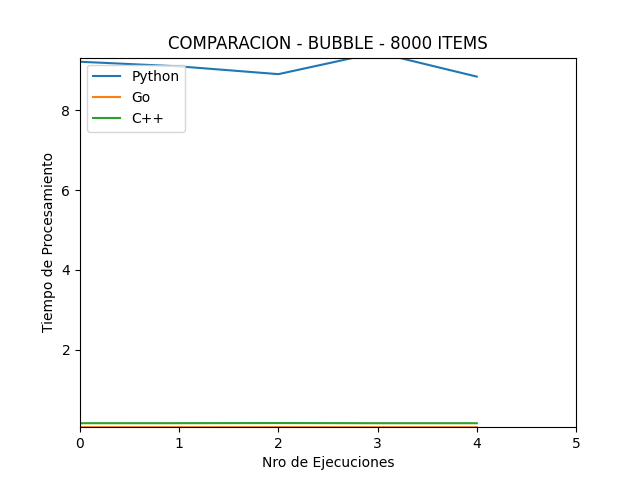
\includegraphics[width=\textwidth]{bubble_8000}
    \caption{Bubble Sort - 8000 items}
    \end{figure}

    \vspace{5mm}
    
    \begin{figure}[H]
    \centering
    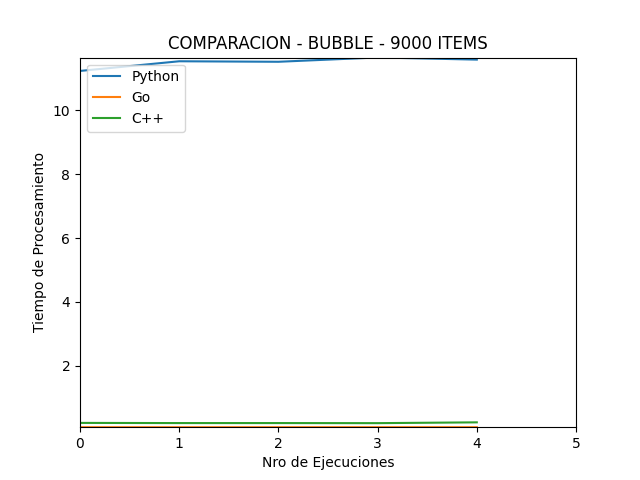
\includegraphics[width=\textwidth]{bubble_9000}
    \caption{Bubble Sort - 9000 items}
    \end{figure}

    \vspace{5mm}
    
    \begin{figure}[H]
    \centering
    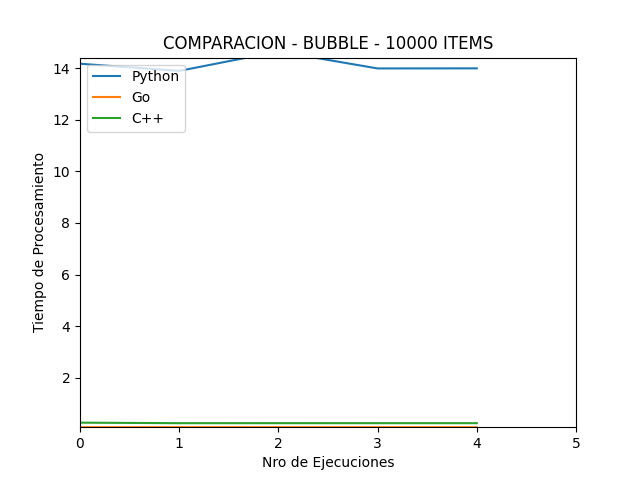
\includegraphics[width=\textwidth]{bubble_10000}
    \caption{Bubble Sort - 10000 items}
    \end{figure}

    \vspace{5mm}
    
    \begin{figure}[H]
    \centering
    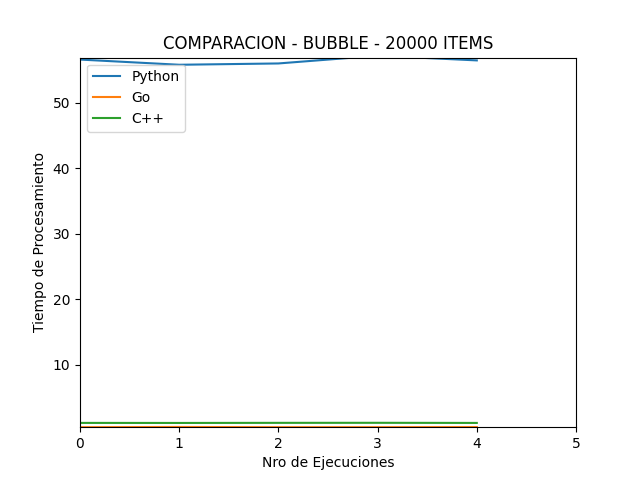
\includegraphics[width=\textwidth]{bubble_20000}
    \caption{Bubble Sort - 20000 items}
    \end{figure}

    \vspace{5mm}
    
    \begin{figure}[H]
    \centering
    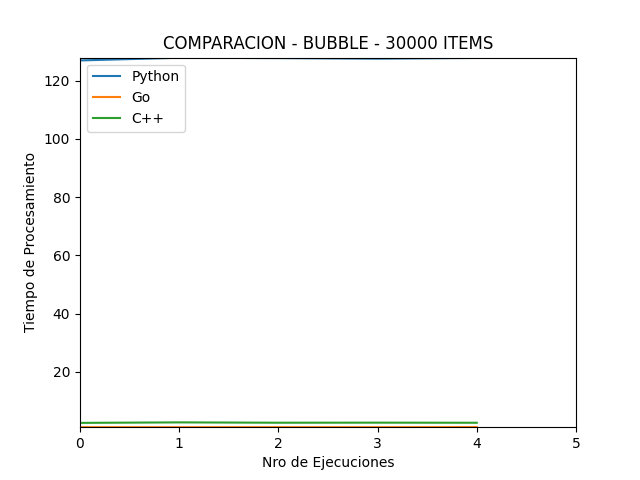
\includegraphics[width=\textwidth]{bubble_30000}
    \caption{Bubble Sort - 30000 items}
    \end{figure}

    \vspace{5mm}
    
    \begin{figure}[H]
    \centering
    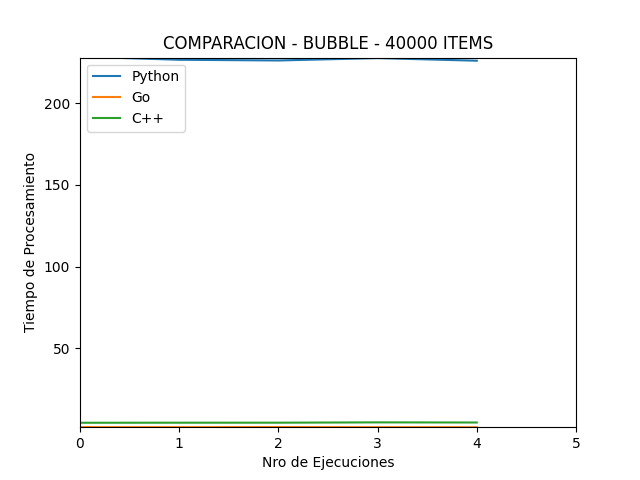
\includegraphics[width=\textwidth]{bubble_40000}
    \caption{Bubble Sort - 40000 items}
    \end{figure}

    \vspace{5mm}
    
    \begin{figure}[H]
    \centering
    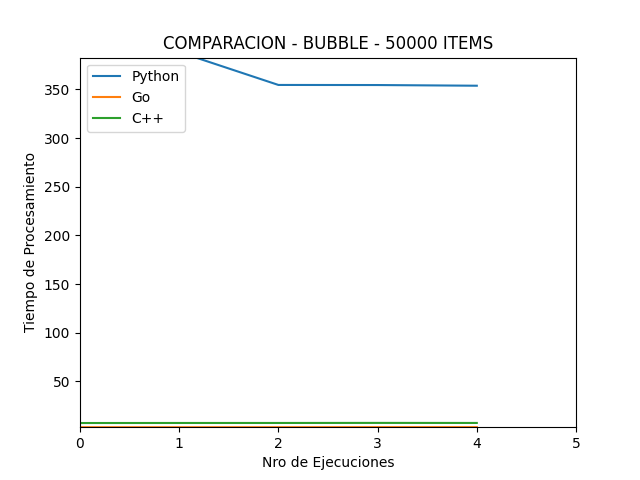
\includegraphics[width=\textwidth]{bubble_50000}
    \caption{Bubble Sort - 50000 items}
    \end{figure}

    \vspace{8cm}

BINARY INSERT SORT

\begin{table}[H]
    \def\arraystretch{1.3}
    \centering
    \begin{tabular}{|l|l|l|l|l|l|l|}
    \hline        
        DATOS & Python & ~ & C++ & ~ & Golang & ~ \\ \hline
        Cantidad & Promedio & Desv. Est. & Promedio & Desv. Est. & Promedio & Desv. Est. \\ \hline
        100 & 0.001179 & 0.000412 & 0.000567 & 0.000165 & 0.000227 & 0.000278 \\ \hline
        1000 & 0.011801 & 0.0004 & 0.001388 & 0.000204 & 0.001113 & 0.001147 \\ \hline
        2000 & 0.036404 & 0.000486 & 0.00277 & 0.0002 & 0.00188 & 0.000297 \\ \hline
        3000 & 0.077004 & 0.000543 & 0.004932 & 0.000198 & 0.003172 & 0.000225 \\ \hline
        4000 & 0.146665 & 0.007182 & 0.00784 & 0.000115 & 0.004691 & 0.000264 \\ \hline
        5000 & 0.230609 & 0.00242 & 0.011518 & 0.000306 & 0.006384 & 0.00026 \\ \hline
        6000 & 0.34093 & 0.005628 & 0.017372 & 0.002291 & 0.008773 & 0.000949 \\ \hline
        7000 & 0.467704 & 0.004512 & 0.022372 & 0.002704 & 0.01045 & 0.000267 \\ \hline
        8000 & 0.676307 & 0.045625 & 0.027731 & 0.000381 & 0.013188 & 0.000331 \\ \hline
        9000 & 0.839014 & 0.013345 & 0.03324 & 0.000159 & 0.016326 & 0.000955 \\ \hline
        10000 & 1.095616 & 0.065637 & 0.044264 & 0.005229 & 0.019185 & 0.00045 \\ \hline
        20000 & 4.26201 & 0.03094 & 0.155018 & 0.004108 & 0.062971 & 0.000338 \\ \hline
        30000 & 9.677808 & 0.236474 & 0.345256 & 0.004813 & 0.134754 & 0.002914 \\ \hline
        40000 & 17.100235 & 0.29154 & 0.599238 & 0.006217 & 0.237646 & 0.009486 \\ \hline
        50000 & 27.796896 & 0.641884 & 0.945106 & 0.010825 & 0.357538 & 0.012083 \\ \hline
    \end{tabular}
    \caption{Tabla de Promedios y Desviacion Estandar de los 3 lenguajes con Binary Insertion Sort}
\end{table}

\vspace{6cm}



\begin{figure}[H]
    \centering
    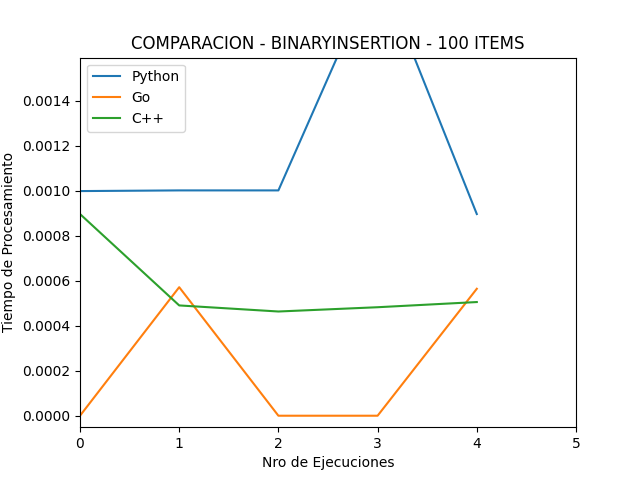
\includegraphics[width=\textwidth]{binaryInsertion_100}
    \caption{Binary Insert Sort - 100 items}
    \end{figure}
    
    \vspace{5mm}
    
    \begin{figure}[H]
    \centering
    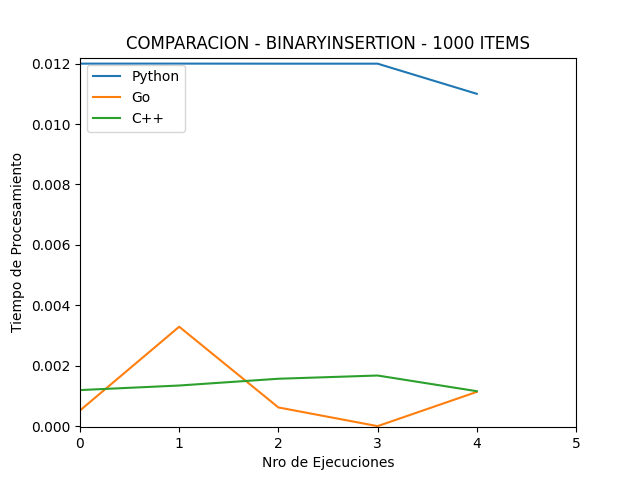
\includegraphics[width=\textwidth]{binaryInsertion_1000}
    \caption{Binary Insert Sort - 1000 items}
    \end{figure}
    
    \vspace{5mm}
    
    \begin{figure}[H]
    \centering
    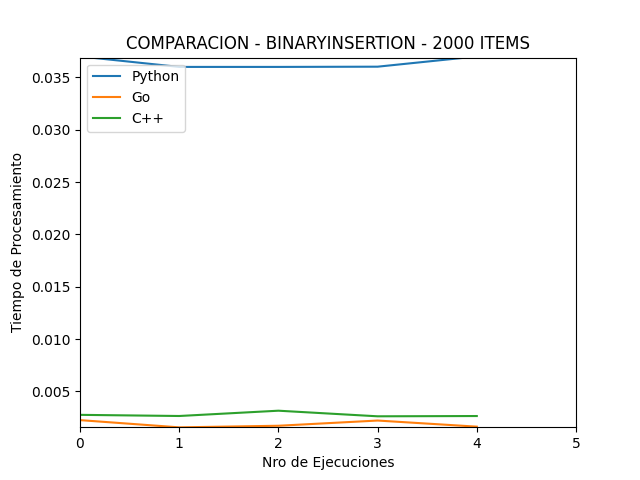
\includegraphics[width=\textwidth]{binaryInsertion_2000}
    \caption{Binary Insert Sort - 2000 items}
    \end{figure}
    
    \vspace{5mm}
    
    \begin{figure}[H]
    \centering
    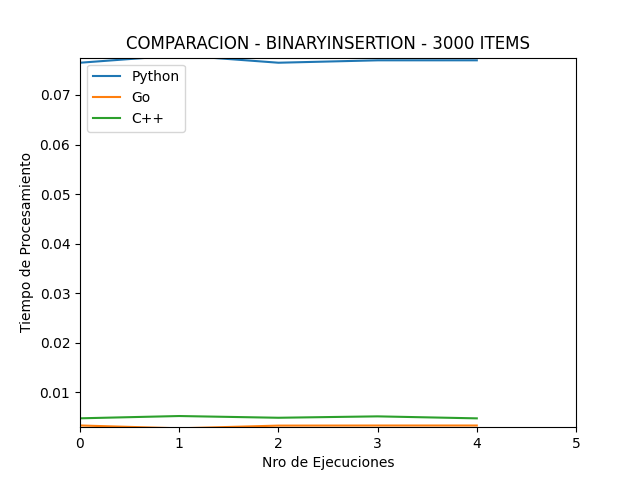
\includegraphics[width=\textwidth]{binaryInsertion_3000}
    \caption{Binary Insert Sort - 3000 items}
    \end{figure}
    
    \vspace{5mm}
    
    \begin{figure}[H]
    \centering
    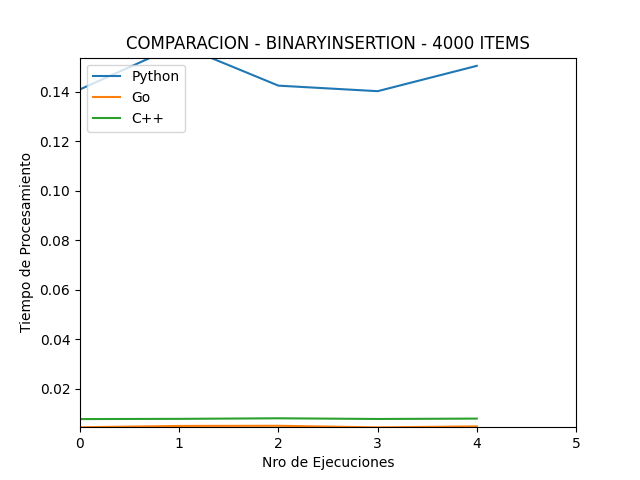
\includegraphics[width=\textwidth]{binaryInsertion_4000}
    \caption{Binary Insert Sort - 4000 items}
    \end{figure}

    \vspace{5mm}
    
    \begin{figure}[H]
    \centering
    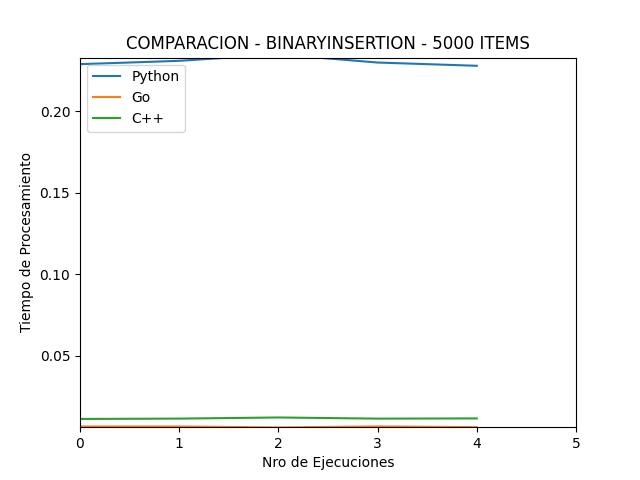
\includegraphics[width=\textwidth]{binaryInsertion_5000}
    \caption{Binary Insert Sort - 5000 items}
    \end{figure}

    \vspace{5mm}
    
    \begin{figure}[H]
    \centering
    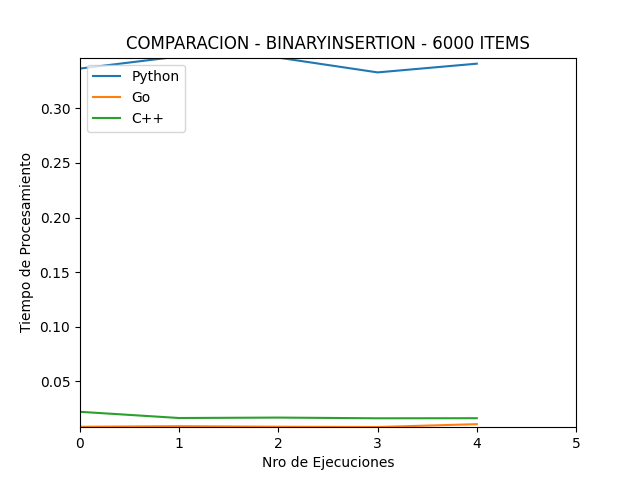
\includegraphics[width=\textwidth]{binaryInsertion_6000}
    \caption{Binary Insert Sort - 6000 items}
    \end{figure}

    \vspace{5mm}
    
    \begin{figure}[H]
    \centering
    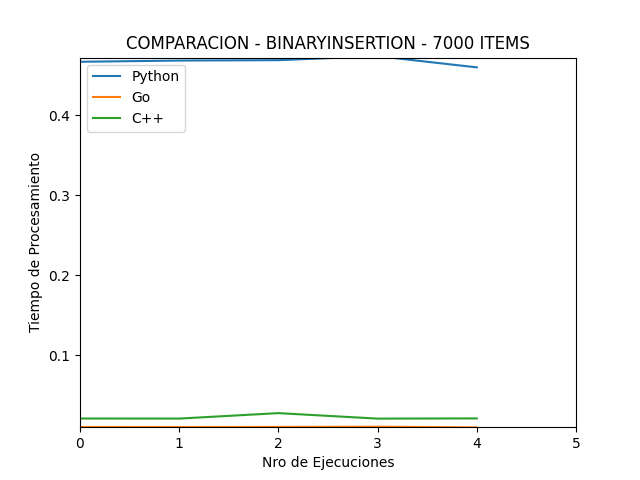
\includegraphics[width=\textwidth]{binaryInsertion_7000}
    \caption{Binary Insert Sort - 7000 items}
    \end{figure}

    \vspace{5mm}
    
    \begin{figure}[H]
    \centering
    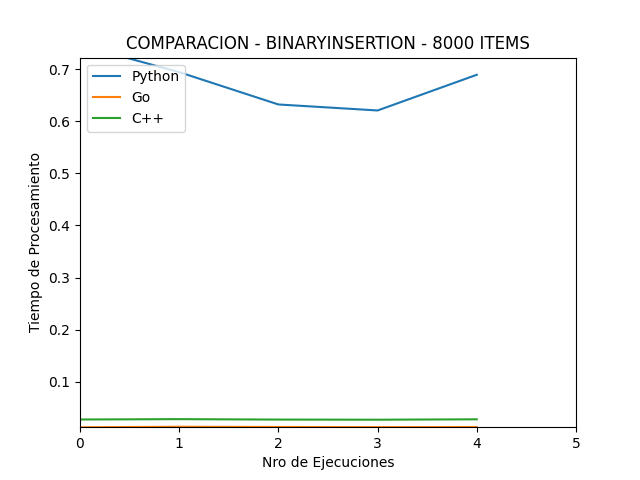
\includegraphics[width=\textwidth]{binaryInsertion_8000}
    \caption{Binary Insert Sort - 8000 items}
    \end{figure}

    \vspace{5mm}
    
    \begin{figure}[H]
    \centering
    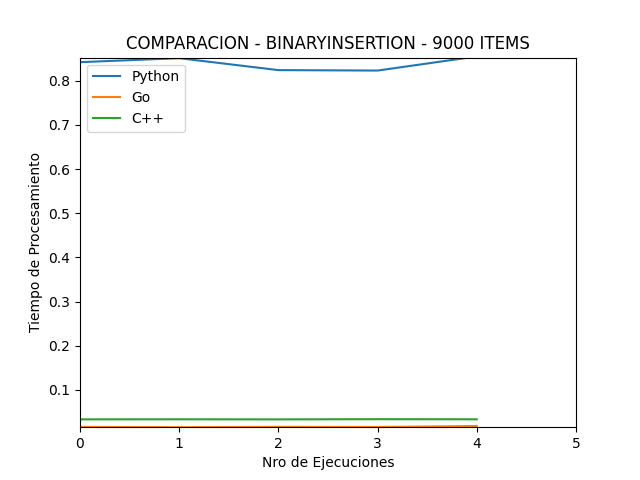
\includegraphics[width=\textwidth]{binaryInsertion_9000}
    \caption{Binary Insert Sort - 9000 items}
    \end{figure}

    \vspace{5mm}
    
    \begin{figure}[H]
    \centering
    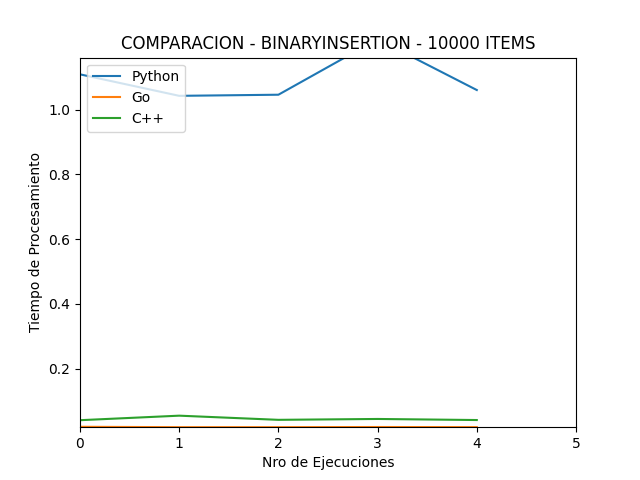
\includegraphics[width=\textwidth]{binaryInsertion_10000}
    \caption{Binary Insert Sort - 10000 items}
    \end{figure}

    \vspace{5mm}
    
    \begin{figure}[H]
    \centering
    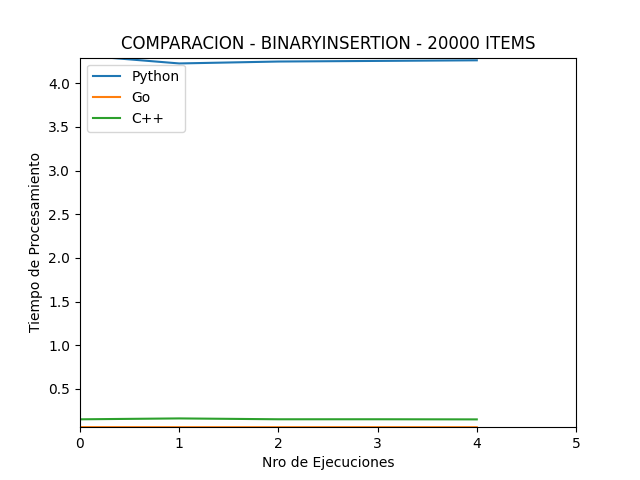
\includegraphics[width=\textwidth]{binaryInsertion_20000}
    \caption{Binary Insert Sort - 20000 items}
    \end{figure}

    \vspace{5mm}
    
    \begin{figure}[H]
    \centering
    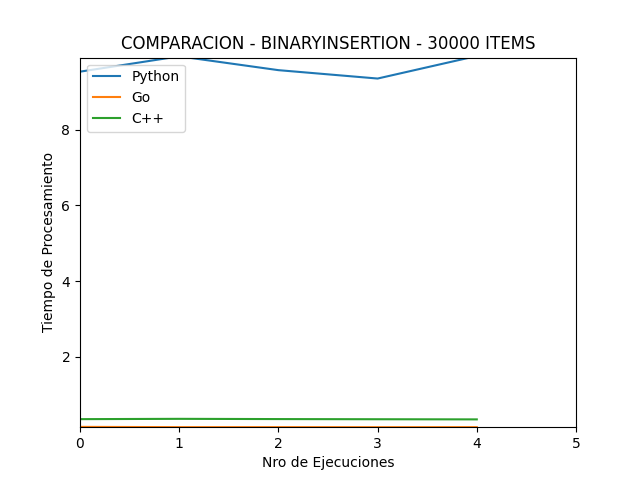
\includegraphics[width=\textwidth]{binaryInsertion_30000}
    \caption{Binary Insert Sort - 30000 items}
    \end{figure}

    \vspace{5mm}
    
    \begin{figure}[H]
    \centering
    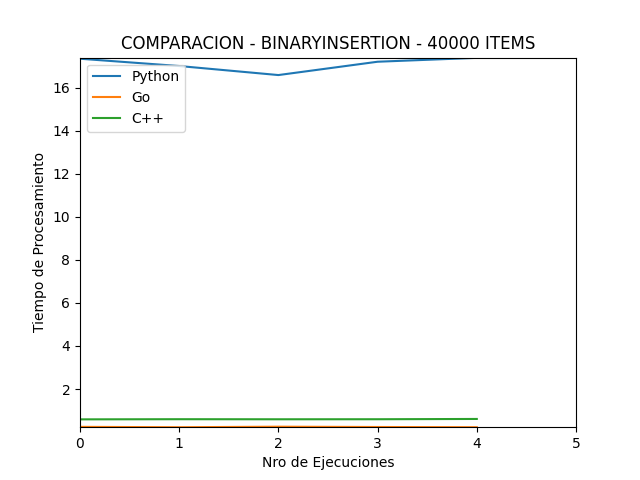
\includegraphics[width=\textwidth]{binaryInsertion_40000}
    \caption{Binary Insert Sort - 40000 items}
    \end{figure}

    \vspace{5mm}
    
    \begin{figure}[H]
    \centering
    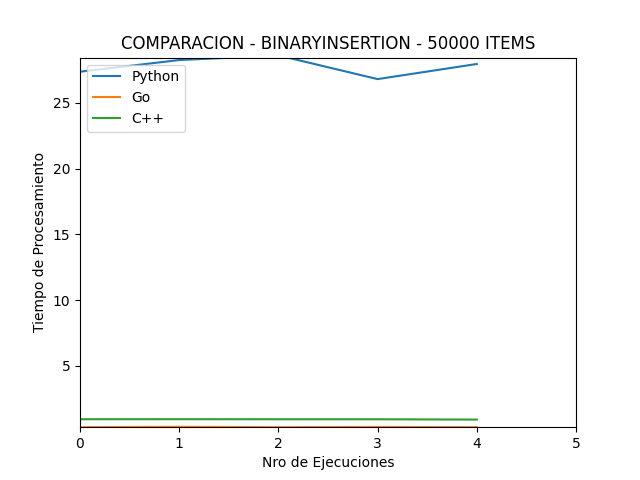
\includegraphics[width=\textwidth]{binaryInsertion_50000}
    \caption{Binary Insert Sort - 50000 items}
    \end{figure}

    \vspace{8cm}

MERGE SORT

\begin{table}[H]
    \def\arraystretch{1.3}
    \centering
    \begin{tabular}{|l|l|l|l|l|l|l|}
    \hline        
        DATOS & Python & ~ & C++ & ~ & Golang & ~ \\ \hline
        Cantidad & Promedio & Desv. Est. & Promedio & Desv. Est. & Promedio & Desv. Est. \\ \hline
        100 & 0.0006 & 0.00049 & 0.000533 & 0.000034 & 0.000429 & 0.000367 \\ \hline
        1000 & 0.003 & 0.000001 & 0.000923 & 0.000036 & 0.000971 & 0.000206 \\ \hline
        2000 & 0.0074 & 0.000491 & 0.001465 & 0.00009 & 0.00162 & 0.000278 \\ \hline
        3000 & 0.0118 & 0.0004 & 0.001893 & 0.00005 & 0.002489 & 0.000452 \\ \hline
        4000 & 0.0162 & 0.001469 & 0.002358 & 0.000061 & 0.003235 & 0.000381 \\ \hline
        5000 & 0.0214 & 0.001358 & 0.00309 & 0.000373 & 0.004025 & 0.000274 \\ \hline
        6000 & 0.053601 & 0.027376 & 0.003449 & 0.000175 & 0.005202 & 0.000436 \\ \hline
        7000 & 0.0302 & 0.0004 & 0.00626 & 0.004867 & 0.005494 & 0.000316 \\ \hline
        8000 & 0.038199 & 0.004167 & 0.004378 & 0.000259 & 0.006255 & 0.000319 \\ \hline
        9000 & 0.043999 & 0.007043 & 0.005047 & 0.000189 & 0.008111 & 0.00061 \\ \hline
        10000 & 0.045199 & 0.0004 & 0.005335 & 0.000297 & 0.008815 & 0.000114 \\ \hline
        20000 & 0.0988 & 0.005601 & 0.010452 & 0.000529 & 0.017305 & 0.002439 \\ \hline
        30000 & 0.153799 & 0.007222 & 0.015751 & 0.000578 & 0.023033 & 0.000283 \\ \hline
        40000 & 0.2198 & 0.018808 & 0.020355 & 0.000142 & 0.030863 & 0.000457 \\ \hline
        50000 & 0.263199 & 0.000748 & 0.025606 & 0.000265 & 0.038622 & 0.001223 \\ \hline
    \end{tabular}
    \caption{Tabla de Promedios y Desviacion Estandar de los 3 lenguajes con Merge Sort}
\end{table}

\vspace{6cm}

\begin{figure}[H]
    \centering
    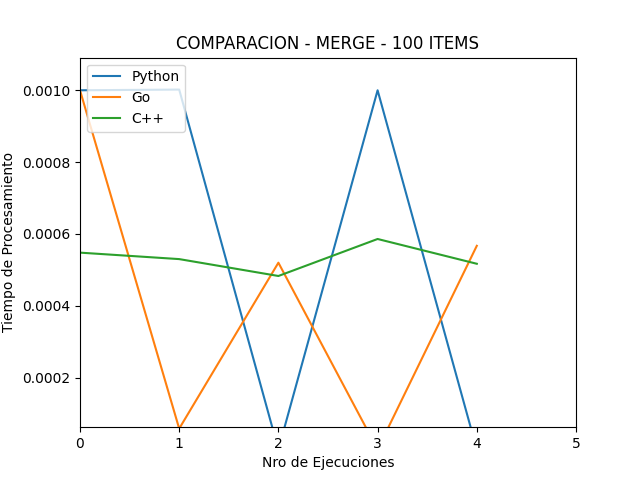
\includegraphics[width=\textwidth]{merge_100}
    \caption{Merge Sort - 100 items}
    \end{figure}
    
    \vspace{5mm}
    
    \begin{figure}[H]
    \centering
    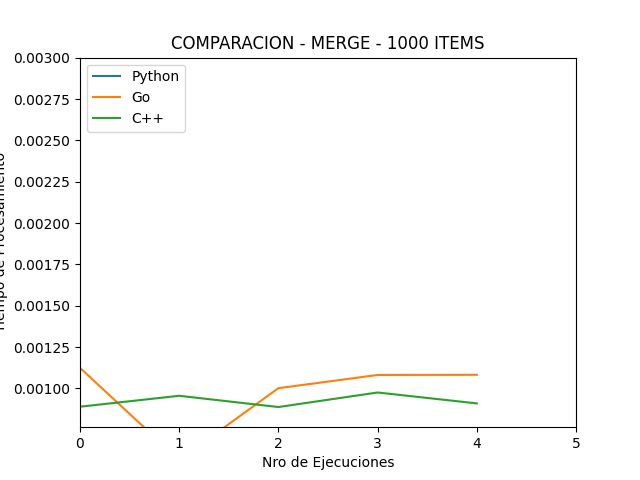
\includegraphics[width=\textwidth]{merge_1000}
    \caption{Merge Sort - 1000 items}
    \end{figure}
    
    \vspace{5mm}
    
    \begin{figure}[H]
    \centering
    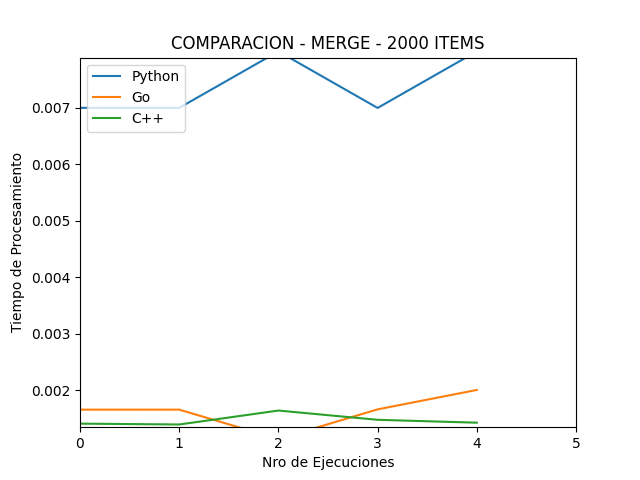
\includegraphics[width=\textwidth]{merge_2000}
    \caption{Merge Sort - 2000 items}
    \end{figure}
    
    \vspace{5mm}
    
    \begin{figure}[H]
    \centering
    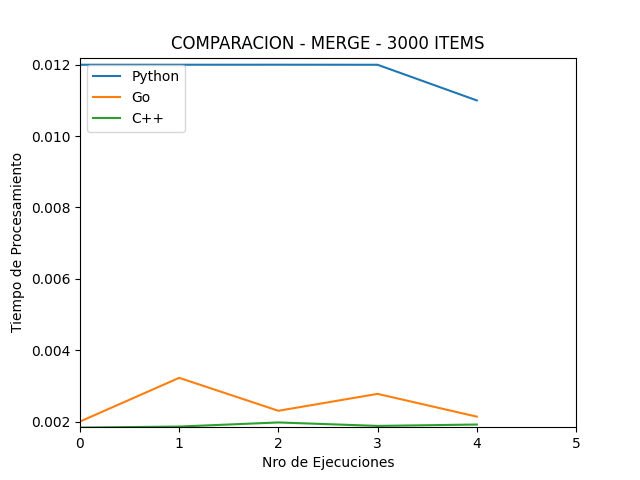
\includegraphics[width=\textwidth]{merge_3000}
    \caption{Merge Sort - 3000 items}
    \end{figure}
    
    \vspace{5mm}
    
    \begin{figure}[H]
    \centering
    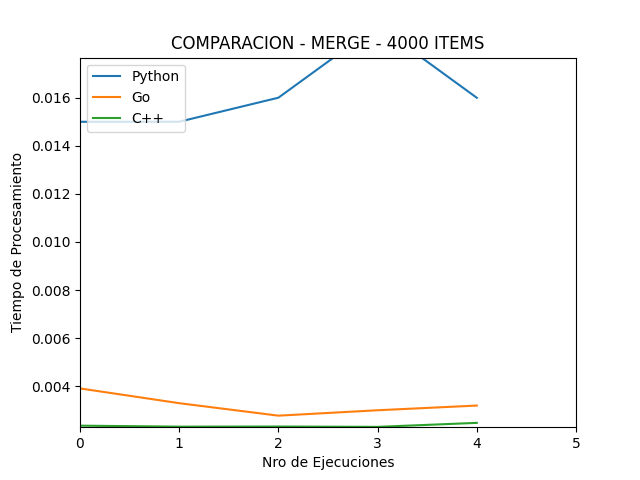
\includegraphics[width=\textwidth]{merge_4000}
    \caption{Merge Sort - 4000 items}
    \end{figure}

    \vspace{5mm}
    
    \begin{figure}[H]
    \centering
    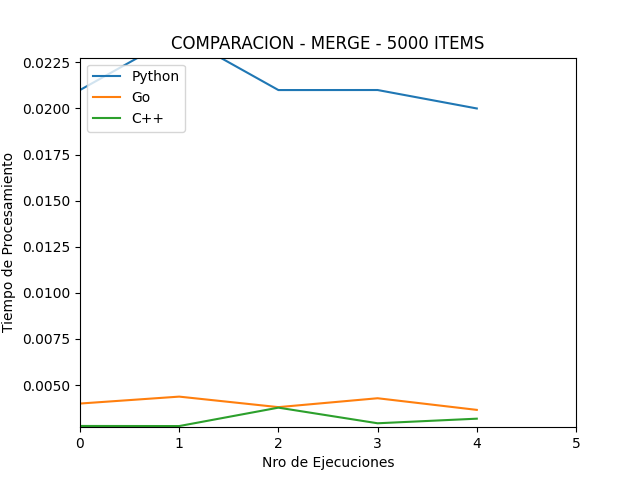
\includegraphics[width=\textwidth]{merge_5000}
    \caption{Merge Sort - 5000 items}
    \end{figure}

    \vspace{5mm}
    
    \begin{figure}[H]
    \centering
    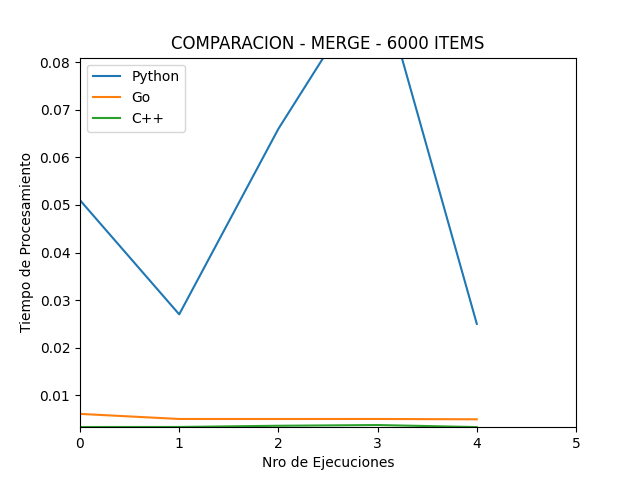
\includegraphics[width=\textwidth]{merge_6000}
    \caption{Merge Sort - 6000 items}
    \end{figure}

    \vspace{5mm}
    
    \begin{figure}[H]
    \centering
    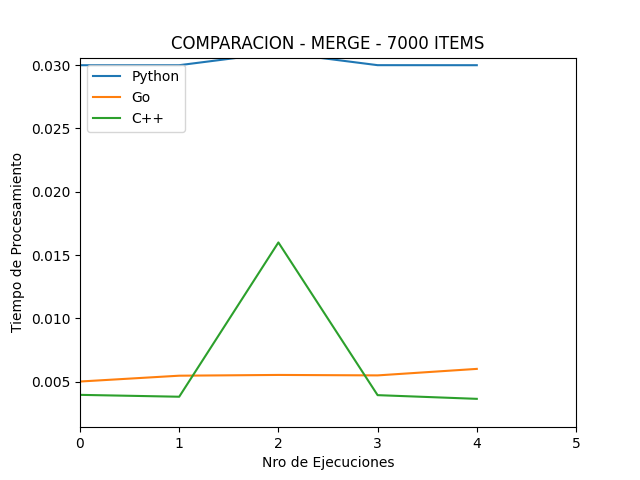
\includegraphics[width=\textwidth]{merge_7000}
    \caption{Merge Sort - 7000 items}
    \end{figure}

    \vspace{5mm}
    
    \begin{figure}[H]
    \centering
    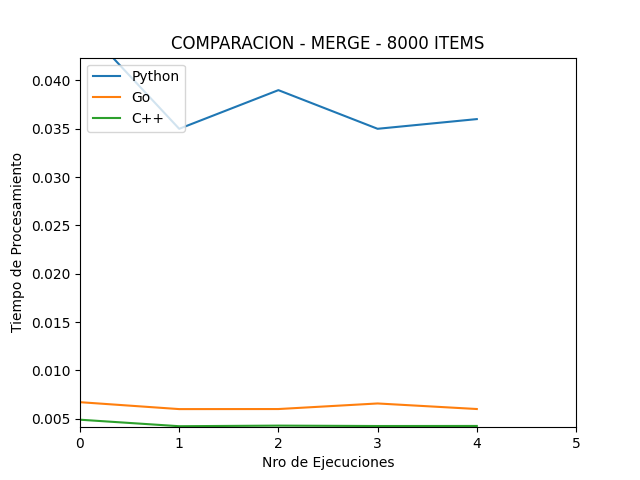
\includegraphics[width=\textwidth]{merge_8000}
    \caption{Merge Sort - 8000 items}
    \end{figure}

    \vspace{5mm}
    
    \begin{figure}[H]
    \centering
    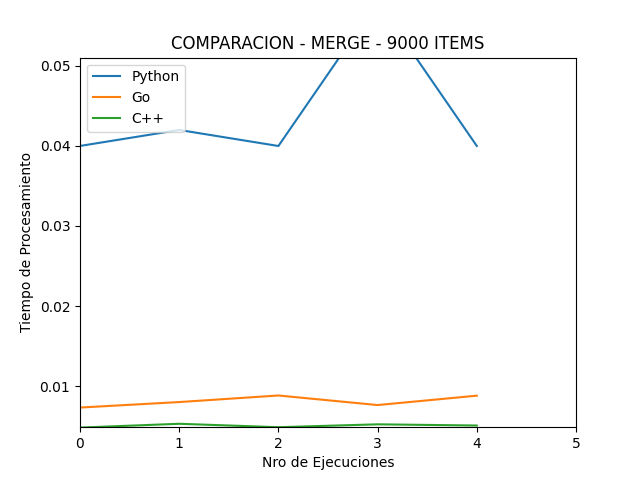
\includegraphics[width=\textwidth]{merge_9000}
    \caption{Merge Sort - 9000 items}
    \end{figure}

    \vspace{5mm}
    
    \begin{figure}[H]
    \centering
    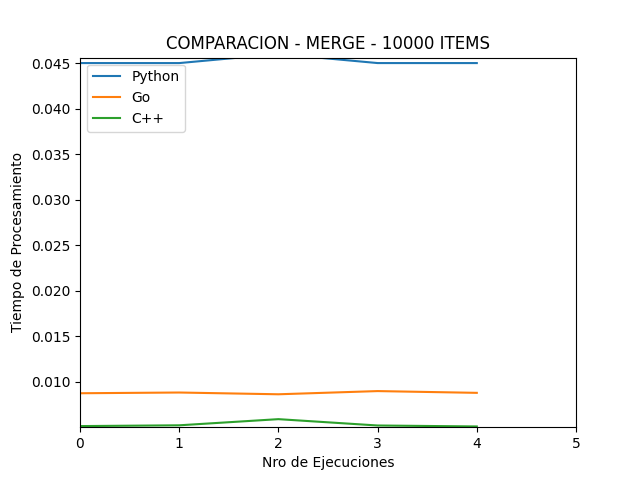
\includegraphics[width=\textwidth]{merge_10000}
    \caption{Merge Sort - 10000 items}
    \end{figure}

    \vspace{5mm}
    
    \begin{figure}[H]
    \centering
    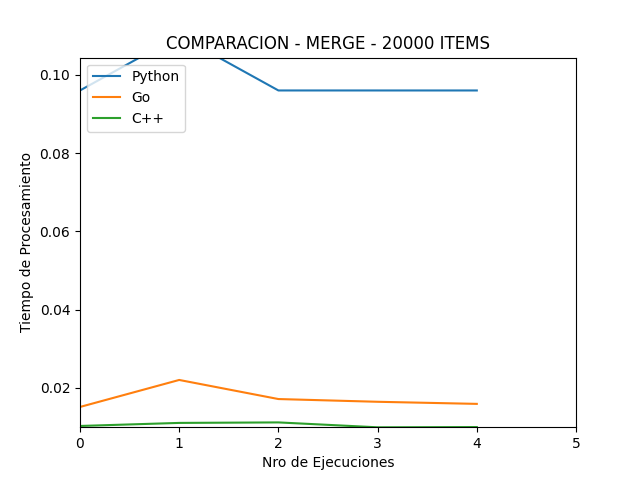
\includegraphics[width=\textwidth]{merge_20000}
    \caption{Merge Sort - 20000 items}
    \end{figure}

    \vspace{5mm}
    
    \begin{figure}[H]
    \centering
    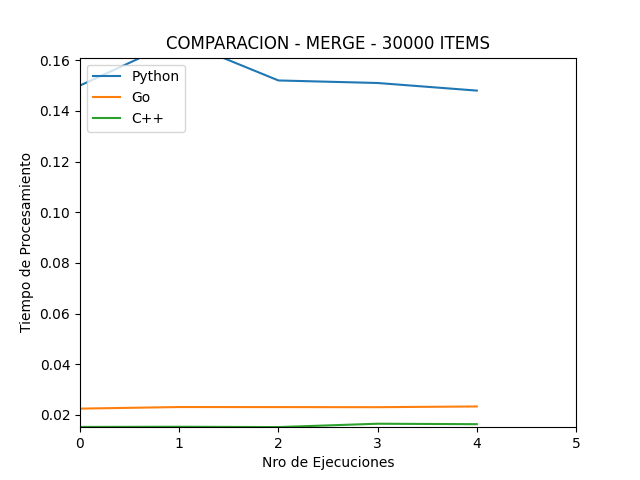
\includegraphics[width=\textwidth]{merge_30000}
    \caption{Merge Sort - 30000 items}
    \end{figure}

    \vspace{5mm}
    
    \begin{figure}[H]
    \centering
    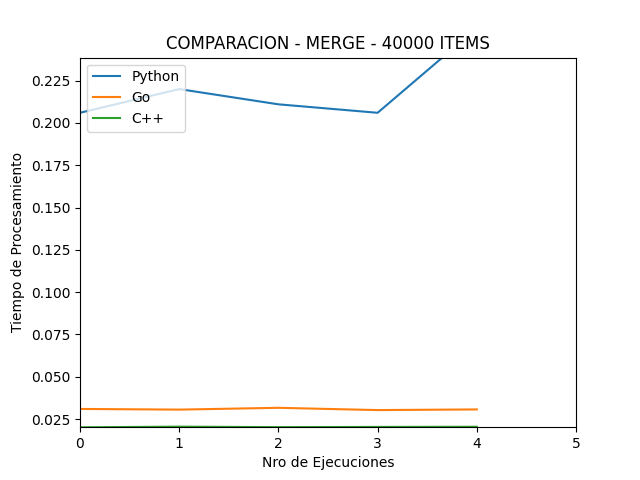
\includegraphics[width=\textwidth]{merge_40000}
    \caption{Merge Sort - 40000 items}
    \end{figure}

    \vspace{5mm}
    
    \begin{figure}[H]
    \centering
    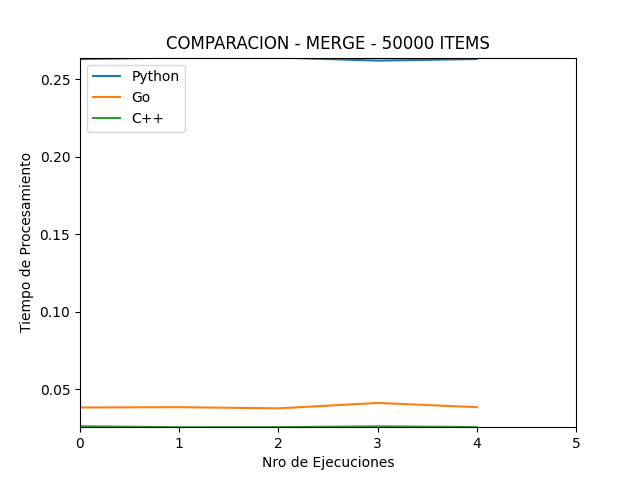
\includegraphics[width=\textwidth]{merge_50000}
    \caption{Merge Sort - 50000 items}
    \end{figure}

    \vspace{8cm}




QUICK SORT

\begin{table}[H]
    \def\arraystretch{1.3}
    \centering
    \begin{tabular}{|l|l|l|l|l|l|l|}
    \hline        
        DATOS & Python & ~ & C++ & ~ & Golang & ~ \\ \hline
        Cantidad & Promedio & Desv. Est. & Promedio & Desv. Est. & Promedio & Desv. Est. \\ \hline
        100 & 0.000993 & 0.000015 & 0.000505 & 0.000049 & 0.000233 & 0.000262 \\ \hline
        1000 & 0.0092 & 0.0064 & 0.00085 & 0.000052 & 0.000694 & 0.000202 \\ \hline
        2000 & 0.0176 & 0.00933 & 0.001574 & 0.000481 & 0.002188 & 0.001663 \\ \hline
        3000 & 0.020801 & 0.000748 & 0.001696 & 0.000126 & 0.001742 & 0.000207 \\ \hline
        4000 & 0.0284 & 0.0048 & 0.003398 & 0.002469 & 0.002316 & 0.000223 \\ \hline
        5000 & 0.04 & 0.012538 & 0.002429 & 0.000055 & 0.003177 & 0.00019 \\ \hline
        6000 & 0.041799 & 0.001166 & 0.002925 & 0.000124 & 0.003416 & 0.000159 \\ \hline
        7000 & 0.052201 & 0.003543 & 0.003394 & 0.000218 & 0.004177 & 0.000253 \\ \hline
        8000 & 0.056599 & 0.001356 & 0.003988 & 0.000487 & 0.004597 & 0.000297 \\ \hline
        9000 & 0.065 & 0.000895 & 0.00412 & 0.000181 & 0.005236 & 0.000265 \\ \hline
        10000 & 0.074599 & 0.0012 & 0.0047 & 0.00029 & 0.005903 & 0.000202 \\ \hline
        20000 & 0.1538 & 0.000749 & 0.009062 & 0.000274 & 0.011642 & 0.00019 \\ \hline
        30000 & 0.257399 & 0.024021 & 0.01318 & 0.000115 & 0.018196 & 0.000386 \\ \hline
        40000 & 0.341 & 0.022135 & 0.01858 & 0.001031 & 0.023219 & 0.000234 \\ \hline
        50000 & 0.431598 & 0.001743 & 0.022693 & 0.001548 & 0.030996 & 0.003827 \\ \hline
    \end{tabular}
    \caption{Tabla de Promedios y Desviacion Estandar de los 3 lenguajes con Quick Sort}
\end{table}

\vspace{10cm}

\begin{figure}[H]
    \centering
    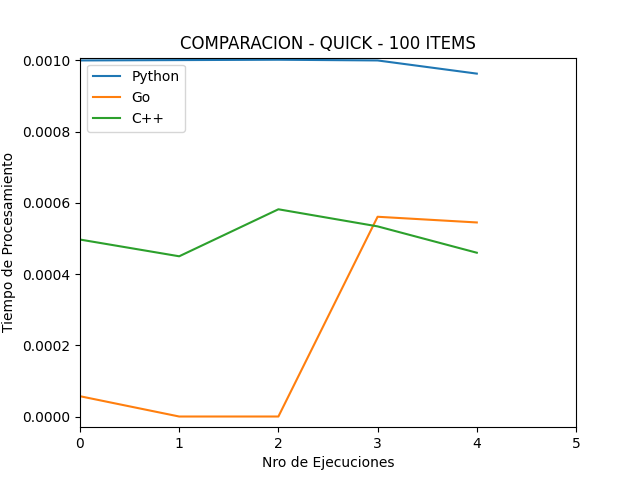
\includegraphics[width=\textwidth]{quick_100}
    \caption{Quick Sort - 100 items}
    \end{figure}
    
    \vspace{5mm}
    
    \begin{figure}[H]
    \centering
    \includegraphics[width=\textwidth]{quick_1000}
    \caption{Quick Sort - 1000 items}
    \end{figure}
    
    \vspace{5mm}
    
    \begin{figure}[H]
    \centering
    \includegraphics[width=\textwidth]{quick_2000}
    \caption{Quick Sort - 2000 items}
    \end{figure}
    
    \vspace{5mm}
    
    \begin{figure}[H]
    \centering
    \includegraphics[width=\textwidth]{quick_3000}
    \caption{Quick Sort - 3000 items}
    \end{figure}
    
    \vspace{5mm}
    
    \begin{figure}[H]
    \centering
    \includegraphics[width=\textwidth]{quick_4000}
    \caption{Quick Sort - 4000 items}
    \end{figure}

    \vspace{5mm}
    
    \begin{figure}[H]
    \centering
    \includegraphics[width=\textwidth]{quick_5000}
    \caption{Quick Sort - 5000 items}
    \end{figure}

    \vspace{5mm}
    
    \begin{figure}[H]
    \centering
    \includegraphics[width=\textwidth]{quick_6000}
    \caption{Quick Sort - 6000 items}
    \end{figure}

    \vspace{5mm}
    
    \begin{figure}[H]
    \centering
    \includegraphics[width=\textwidth]{quick_7000}
    \caption{Quick Sort - 7000 items}
    \end{figure}

    \vspace{5mm}
    
    \begin{figure}[H]
    \centering
    \includegraphics[width=\textwidth]{quick_8000}
    \caption{Quick Sort - 8000 items}
    \end{figure}

    \vspace{5mm}
    
    \begin{figure}[H]
    \centering
    \includegraphics[width=\textwidth]{quick_9000}
    \caption{Quick Sort - 9000 items}
    \end{figure}

    \vspace{5mm}
    
    \begin{figure}[H]
    \centering
    \includegraphics[width=\textwidth]{quick_10000}
    \caption{Quick Sort - 10000 items}
    \end{figure}

    \vspace{5mm}
    
    \begin{figure}[H]
    \centering
    \includegraphics[width=\textwidth]{quick_20000}
    \caption{Quick Sort - 20000 items}
    \end{figure}

    \vspace{5mm}
    
    \begin{figure}[H]
    \centering
    \includegraphics[width=\textwidth]{quick_30000}
    \caption{Quick Sort - 30000 items}
    \end{figure}

    \vspace{5mm}
    
    \begin{figure}[H]
    \centering
    \includegraphics[width=\textwidth]{quick_40000}
    \caption{Quick Sort - 40000 items}
    \end{figure}

    \vspace{5mm}
    
    \begin{figure}[H]
    \centering
    \includegraphics[width=\textwidth]{quick_50000}
    \caption{Quick Sort - 50000 items}
    \end{figure}

    \vspace{8cm}










SELECTION SORT

\begin{table}[H]
    \def\arraystretch{1.3}
    \centering
    \begin{tabular}{|l|l|l|l|l|l|l|}
    \hline        
        DATOS & Python & ~ & C++ & ~ & Golang & ~ \\ \hline
        Cantidad & Promedio & Desv. Est. & Promedio & Desv. Est. & Promedio & Desv. Est. \\ \hline
        100 & 0.001999 & 0.000001 & 0.000531 & 0.000029 & 0.000422 & 0.000212 \\ \hline
        1000 & 0.201399 & 0.066018 & 0.006025 & 0.008607 & 0.001102 & 0.000024 \\ \hline
        2000 & 0.6088 & 0.014274 & 0.008384 & 0.005724 & 0.004712 & 0.002605 \\ \hline
        3000 & 1.3838 & 0.049297 & 0.017627 & 0.013963 & 0.008327 & 0.000347 \\ \hline
        4000 & 2.465399 & 0.056237 & 0.02121 & 0.006782 & 0.015216 & 0.000272 \\ \hline
        5000 & 3.838001 & 0.071756 & 0.027197 & 0.000474 & 0.023363 & 0.000289 \\ \hline
        6000 & 5.5782 & 0.167367 & 0.039137 & 0.00143 & 0.039792 & 0.006679 \\ \hline
        7000 & 7.695804 & 0.399161 & 0.051664 & 0.000391 & 0.05184 & 0.000344 \\ \hline
        8000 & 10.266799 & 0.444722 & 0.066706 & 0.000557 & 0.074552 & 0.003197 \\ \hline
        9000 & 12.484799 & 0.234154 & 0.083624 & 0.000264 & 0.099216 & 0.012354 \\ \hline
        10000 & 15.568 & 0.241852 & 0.10276 & 0.000199 & 0.114273 & 0.000478 \\ \hline
        20000 & 62.645672 & 1.58434 & 0.403848 & 0.00289 & 0.516882 & 0.005456 \\ \hline
        30000 & 143.626945 & 5.320718 & 0.902256 & 0.003313 & 1.176029 & 0.01479 \\ \hline
        40000 & 259.757819 & 13.970079 & 1.652836 & 0.04999 & 2.139661 & 0.048178 \\ \hline
        50000 & 385.468399 & 3.933536 & 2.551786 & 0.093821 & 3.354922 & 0.037221 \\ \hline
    \end{tabular}
    \caption{Tabla de Promedios y Desviacion Estandar de los 3 lenguajes con Selection Sort}
\end{table}

\vspace{10cm}

\begin{figure}[H]
    \centering
    \includegraphics[width=\textwidth]{selection_100}
    \caption{Selection Sort - 100 items}
    \end{figure}
    
    \vspace{5mm}
    
    \begin{figure}[H]
    \centering
    \includegraphics[width=\textwidth]{selection_1000}
    \caption{Selection Sort - 1000 items}
    \end{figure}
    
    \vspace{5mm}
    
    \begin{figure}[H]
    \centering
    \includegraphics[width=\textwidth]{selection_2000}
    \caption{Selection Sort - 2000 items}
    \end{figure}
    
    \vspace{5mm}
    
    \begin{figure}[H]
    \centering
    \includegraphics[width=\textwidth]{selection_3000}
    \caption{Selection Sort - 3000 items}
    \end{figure}
    
    \vspace{5mm}
    
    \begin{figure}[H]
    \centering
    \includegraphics[width=\textwidth]{selection_4000}
    \caption{Selection Sort - 4000 items}
    \end{figure}

    \vspace{5mm}
    
    \begin{figure}[H]
    \centering
    \includegraphics[width=\textwidth]{selection_5000}
    \caption{Selection Sort - 5000 items}
    \end{figure}

    \vspace{5mm}
    
    \begin{figure}[H]
    \centering
    \includegraphics[width=\textwidth]{selection_6000}
    \caption{Selection Sort - 6000 items}
    \end{figure}

    \vspace{5mm}
    
    \begin{figure}[H]
    \centering
    \includegraphics[width=\textwidth]{selection_7000}
    \caption{Selection Sort - 7000 items}
    \end{figure}

    \vspace{5mm}
    
    \begin{figure}[H]
    \centering
    \includegraphics[width=\textwidth]{selection_8000}
    \caption{Selection Sort - 8000 items}
    \end{figure}

    \vspace{5mm}
    
    \begin{figure}[H]
    \centering
    \includegraphics[width=\textwidth]{selection_9000}
    \caption{Selection Sort - 9000 items}
    \end{figure}

    \vspace{5mm}
    
    \begin{figure}[H]
    \centering
    \includegraphics[width=\textwidth]{selection_10000}
    \caption{Selection Sort - 10000 items}
    \end{figure}

    \vspace{5mm}
    
    \begin{figure}[H]
    \centering
    \includegraphics[width=\textwidth]{selection_20000}
    \caption{Selection Sort - 20000 items}
    \end{figure}

    \vspace{5mm}
    
    \begin{figure}[H]
    \centering
    \includegraphics[width=\textwidth]{selection_30000}
    \caption{Selection Sort - 30000 items}
    \end{figure}

    \vspace{5mm}
    
    \begin{figure}[H]
    \centering
    \includegraphics[width=\textwidth]{selection_40000}
    \caption{Selection Sort - 40000 items}
    \end{figure}

    \vspace{5mm}
    
    \begin{figure}[H]
    \centering
    \includegraphics[width=\textwidth]{selection_50000}
    \caption{Selection Sort - 50000 items}
    \end{figure}

    \vspace{8cm}



Como se puede ver en las tablas comparativas, Python llego a necesitar mas de 300 seg para la ejecucion de 50000 datos, sobre todo con algoritmos como BubbleSort y SelectionSort, siendo los de mas complejidad,
Tambien podemos observar que Go y C++ tienen muy similares los tiempos en promedio, siendo los lenguajes mas rapidos incluso en los 2 algoritmos mencionados anteriormente.


\vspace{5mm}

\section{Conclusiones}

Como conclusiones del informe podemos indicar lo siguiente:

\begin{itemize}
    \item En la comparativa de los 5 algoritmos seleccionados, se concluye que quicksort y mergesort son los algoritmos mas rapidos, binary insertion sort seria el que les sigue y bubblesort y selectionsort serian los mas lentos
    segun el tamaño de las listas comparadas
    \item En la comparativa de los 3 lenguajes de programacion: Python, C++ y Golang, Python seria el lenguaje mas lento, mostrando altos tiempos de ejecucion en listas de mayor tamaño, mientras que C++ y Golang serian mas rapidos, manteniendo un margen no mayor a 3 seg incluso en listas de gran tamaño
\end{itemize}
\end{document}